\chapter{Running EVA on the Wheel: A Reproducible Numerical Trace}\label{ch:trace}
\section{The experimental specification}
We now run sequential EVA on $W_6(1)$ using the exact weighted adjacency from \cref{ch:wheel6}, embedding rank $p=4$, the NumPy \texttt{default\_rng} with seed $2026$, independent initial row entries uniform on $[0,1)$ followed by unit normalization, and angular stopping threshold $10^{-6}$. The code in \texttt{code/check\_examples.py} is independently executable and documents every numerical convention. The theoretical optimal objective is already certified analytically as $7.368033988749895\ldots$.

\section{Selected measured epochs}
The following values were obtained by executing the included pure-NumPy reference script; the maximum angle is the largest \emph{within-epoch row update angle}.
\begin{center}\small
\begin{tabular}{r S[table-format=1.9] S[table-format=1.9]}
\toprule
Epoch & {Continuous objective $F(Y)$} & {Maximum update angle (rad)}\\\midrule
1 & 6.262899968 & 2.687626862\\
2 & 7.181066881 & 2.065484440\\
3 & 7.253321824 & 0.291491224\\
5 & 7.348964390 & 0.223502967\\
10 & 7.368029070 & 0.003863030\\
20 & 7.368033989 & 0.000000845\\
\bottomrule
\end{tabular}
\end{center}
\noindent\textit{Note:} The table uses the \texttt{S} column type from \texttt{siunitx}; if unavailable in a stripped-down TeX installation, replace these two columns by ordinary right-aligned \texttt{r} columns. The source's preamble loads the required package.

The objective monotonically approaches the analytically known optimum from below, exactly as the coordinate-ascent argument predicts. The run is \emph{not} itself a formal proof of global convergence; the independent dual construction provides that proof for this particular graph. At the last epoch, the measured objective is $7.368033988749668$; the Frobenius distance between the computed and explicit theoretical Gram matrices is approximately $2.67\times10^{-6}$.

\begin{figure}[ht]
\centering
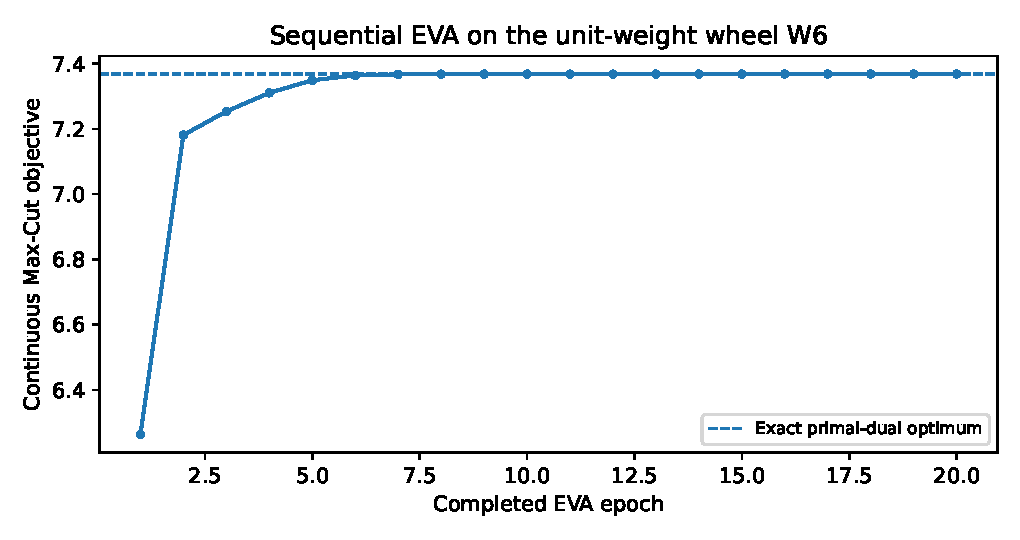
\includegraphics[width=.82\textwidth]{figures/eva_wheel6_trace.pdf}
\caption{An independently regenerated trace of sequential coordinate-ascent EVA on $W_6(1)$ (seed 2026, rank 4); the dashed horizontal line is the analytically certified SDP optimum.}\label{fig:eva-trace}
\end{figure}

\section{Full objective, Gram error, and cut error are different diagnostics}
A small primal objective error does not force the embedding to be close to a unique matrix, since optima may not be unique. The Frobenius discrepancy $\norm{YY^\top-X^*}_F$ is meaningful relative to a specified reference Gram matrix and is rotation invariant. The final rounded cut is a separate random or deterministic object; its value is at most $7$ even when the continuous objective is approximately $7.368$.

\section{An example of rounder quality versus relaxation quality}
For the wheel's exact three-dimensional Gram solution at $q=1$, each rim edge has
\[
X_{i,i+1}=-c+(1+c)(a^*)^2\approx-0.6708203933,
\]
while each spoke has $X_{i,5}=-a^*\approx-0.2763932023$. By the random-hyperplane formula,
\begin{align}
\E[\Cut(x)]&=\frac5\pi\arccos(-0.6708203933)+\frac5\pi\arccos(-0.2763932023)\\
&\approx 6.6159853305.
\end{align}
The theoretical cut optimum is $7$. A strong discrete result can therefore be obtained by selecting the best of several hyperplane samples or applying local improvement after rounding, even though the SDP matrix remains fixed. This is precisely why separating \emph{continuous optimization quality} from \emph{rounding quality} matters.
